\documentclass[a0,portrait]{a0poster}

\usepackage{setspace}
\usepackage{multicol} % This is so we can have multiple columns of text side-by-side
\columnsep=100pt % This is the amount of white space between the columns in the poster
\columnseprule=3pt % This is the thickness of the black line between the columns in the poster

\usepackage[svgnames]{xcolor} % Specify colors by their 'svgnames', for a full list of all colors available see here: http://www.latextemplates.com/svgnames-colors

\usepackage{times} % Use the times font
%\usepackage{palatino} % Uncomment to use the Palatino font

\usepackage{graphicx} % Required for including images
\graphicspath{{figures/}} % Location of the graphics files
\usepackage{booktabs} % Top and bottom rules for table
\usepackage[font=small,labelfont=bf]{caption} % Required for specifying captions to tables and figures
\usepackage{amsfonts, amsmath, amsthm, amssymb} % For math fonts, symbols and environments
\usepackage{wrapfig} % Allows wrapping text around tables and figures
\usepackage{setspace}
\usepackage{subfigure}
\usepackage{commath}
\usepackage{enumerate}
\usepackage{multimedia}
\usepackage{biblatex}



\begin{document}

%----------------------------------------------------------------------------------------
%	POSTER HEADER
%----------------------------------------------------------------------------------------

% The header is divided into two boxes:
% The first is 75% wide and houses the title, subtitle, names, university/organization and contact information
% The second is 25% wide and houses a logo for your university/organization or a photo of you
% The widths of these boxes can be easily edited to accommodate your content as you see fit

\begin{minipage}[b]{\linewidth}

\Huge \color{NavyBlue} \textbf{Numerical simulation of turbulent combustion using turbulent flamelet model} \color{Black}\\ % Title
\vspace{0.5cm}
\Huge\textit{VG500 Poster}\\[-2cm] % Subtitle

\setlength\columnseprule{0pt}
\begin{multicols}{2}
	\huge \textbf{Yu Cang}\\[0.5cm] % Author(s)
	\LARGE UM-SJTU Joint Institute\\[0.4cm] % University/organization
	\Large \texttt{yu.cang@sjtu.edu.cn}\\
	
	\columnbreak

	
\includegraphics[height=6cm]{pic/JI_logo}\\
\end{multicols}


\end{minipage}
%


\vspace{1cm} % A bit of extra whitespace between the header and poster content

%----------------------------------------------------------------------------------------

\begin{multicols}{2} % This is how many columns your poster will be broken into, a portrait poster is generally split into 2 columns

\color{Navy} % Navy color for the abstract

\begin{abstract}

\large Numerical simulation of turbulent combustion is carried out using the turbulent flamelet model. Numerical results, compared with traditional methods, suggest that this new model is well designed for Large Eddy Simulation(LES) and has better agreement with experimental data.

\end{abstract}

\color{SaddleBrown} % SaddleBrown color for the introduction
\section*{Combustor Model}
	\begin{center}
		\vspace{-0.5cm}
		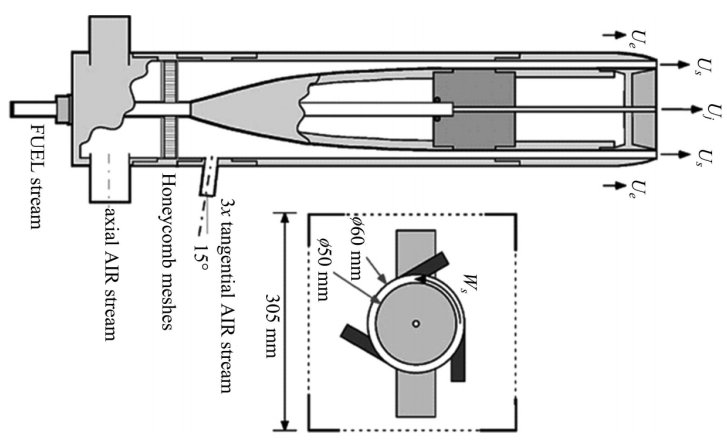
\includegraphics[width=0.8\linewidth]{pic/burner.png}\\
		\vspace{-0.5cm}
		{\color{Green} Fig. 1 Channel Model with Sawtoothed Surface}
	\end{center}

\section*{Governing Equations}
	\color{DarkSlateGray}
    \begin{align}
      \mbox{(Continuity)}\qquad & \frac{\partial \bar{\rho}}{\partial t} + \frac{\partial (\bar{\rho}\tilde{u}_j)}{\partial x_j}=0\\
      \mbox{(Momentum)}\qquad & \dfrac{\partial(\bar{\rho}\tilde{u}_i)}{\partial t} + \dfrac{\partial (\bar{\rho}\tilde{u}_i\tilde{u}_j)}{\partial x_j} = -\dfrac{\partial \bar{p}}{\partial x_i} + 2\dfrac{\partial \bar{\mu}\tilde{S}_{ij}}{\partial x_j} + \dfrac{\partial t_{ij
      }}{\partial x_j}\label{NS}\\
      \mbox{(Scalar transport)}\qquad & \dfrac{\partial(\bar{\rho}\tilde{\phi}_i)}{\partial t} + \dfrac{\partial (\bar{\rho}\tilde{\phi}_i\tilde{u}_j)}{\partial x_j} = \dfrac{\partial \bar{\rho}\tilde{\alpha}_{i}\tilde{\phi}_{i, k}}{\partial x_k} + \bar{\rho}\tilde{\omega}_i + \dfrac{\partial q_{ik
      }}{\partial x_k}
    \end{align}
	where
	\[\tilde{S}_{ij} = \frac{1}{2}(\tilde{u}_{i,j} + \tilde{u}_{j, i}) - \frac{1}{3}\delta_{ij}\tilde{u}_{k,k}\]
	
\color{SaddleBrown}
\section*{Flamelet Assumption}
	\color{DarkSlateGray}
	Locally, the characteristic timescale of chemical reaction is much smaller that that of flow$(t_c \ll t_f)$.\newline
	Thus, local flame structure can be described by the difffusion flame under counterflow configuration.
	\vspace{0.5cm}
	\begin{center}
		\vspace{-0.5cm}
		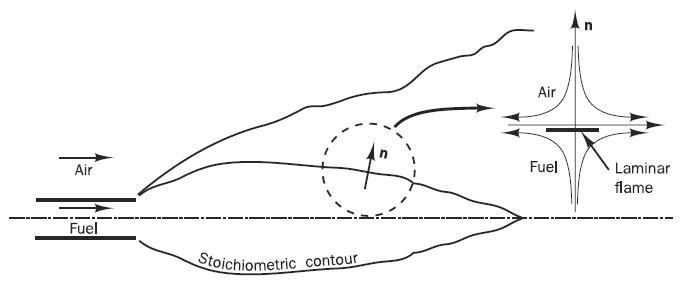
\includegraphics[width=0.85\linewidth]{pic/flamelet.png}\\
		\vspace{-0.25cm}
		{\color{Green} Fig. 2 Local laminar flamelet}
	\end{center}


\color{SaddleBrown}
\section*{Solution Procedure}
	\vspace{-1.5cm}
	\setlength\columnseprule{0pt}
	\begin{multicols}{2}
		\color{DarkSlateGray}
		An iterative process:
		\begin{enumerate}[(1)]
			\item Prepare all properties at $t=n$.
			\item Update flow properties at $t=n+1$ from CFD solver.
			\item Calculate mix-fraction($Z$) and strain-rate($\chi$).
			\item From pre-computed table, lookup temperature($T$) and mass fraction($Y_i$) at $t=n+1$.
			\item Update density($\rho$) at $t=n+1$.
			\item Check convergence.
		\end{enumerate}
		
		\begin{center}
			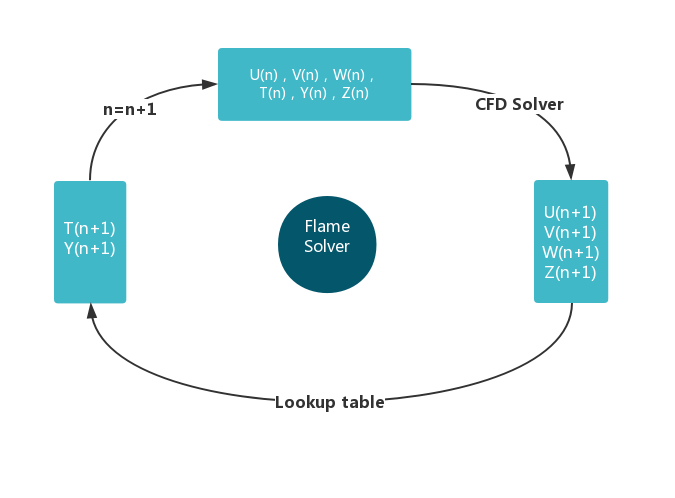
\includegraphics[width=\linewidth]{pic/solver.png}\\
			{\color{Green} Fig. 3 Solution Flowchart}
		\end{center}
	
	\end{multicols}
	\setlength\columnseprule{3pt}

\color{SaddleBrown}
\section*{Grid Layout}
	\vspace{-0.5cm}
	\color{DarkSlateGray}
	Unstructured grid containing tetrahedral, hexahedron and pyramids. Refined locally.
	\vspace{0.5cm}
	\begin{center}
		\vspace{-0.5cm}
		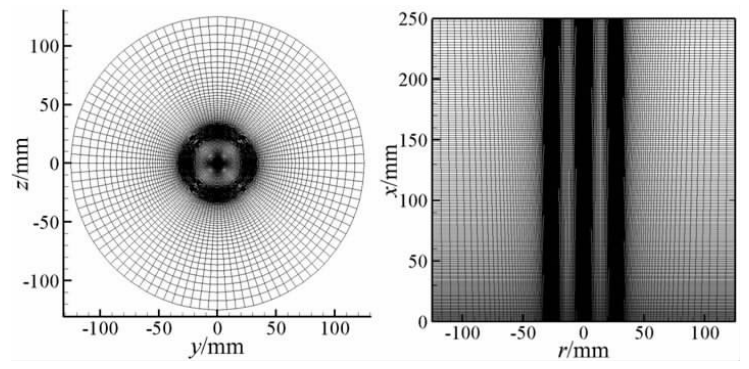
\includegraphics[width=0.55\linewidth]{pic/grid.png}\\
		\vspace{-0.5cm}
		{\color{Green} Fig. 4 Computation grid}
	\end{center}

\color{SaddleBrown}
\section*{Numerical Schemes}
	\vspace{-0.5cm}
	\color{DarkSlateGray}
	Based on the Finite Volume Method(FVM), the intercell flux are computed from 2nd-order upwind schemes. Dynamic subgrid model is adopted in the context of Large Eddy Simulation(LES).

	\setlength\columnseprule{0pt}
	\begin{multicols}{2}
		\color{DarkSlateGray}
		\begin{center}
			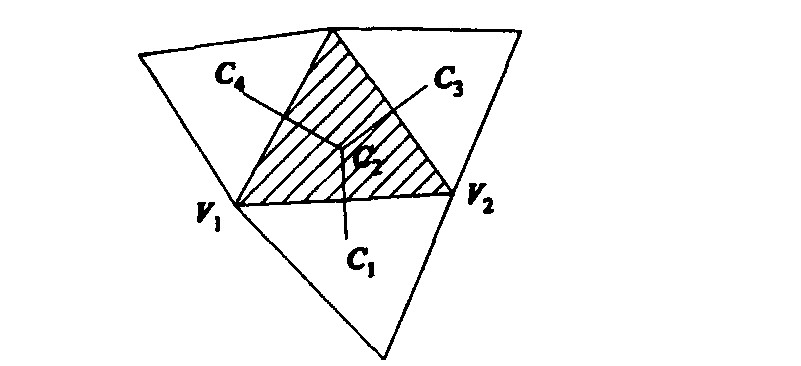
\includegraphics[width=\linewidth]{pic/cell.jpg}\\
			\vspace{0.5cm}
			{\color{Green} Fig. 5 Cell-centered variable}
		\end{center}
		
		\begin{center}
			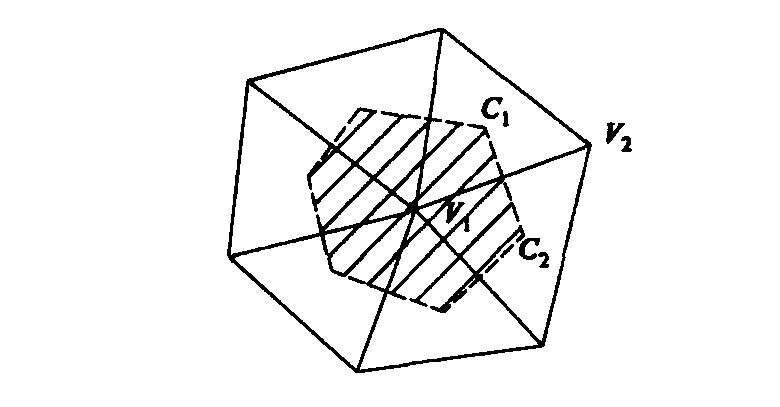
\includegraphics[width=\linewidth]{pic/vertex.jpg}\\
			\vspace{-0.5cm}
			{\color{Green} Fig. 6 Vertex-centered variable}
		\end{center}
	\end{multicols}
	\setlength\columnseprule{3pt}

\color{SaddleBrown}
\section*{Results}
	\color{DarkSlateGray}
	\begin{enumerate}[(1)]
		\item 
			\textbf{The $T_{max}$ plot}.
			\begin{itemize}
				\item 
					One of the most convincing testing cases.
				\item 
					Nice agreement in ignition range compared with reference data.
				\item 
					Difference and transition position are also revealed clearly.	
			\end{itemize}
			\begin{center}
				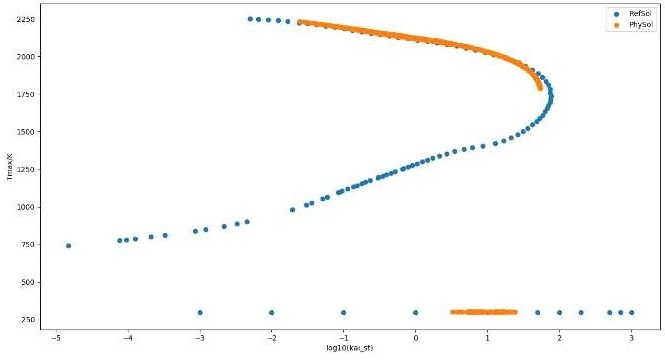
\includegraphics[width=\linewidth]{pic/Tmax.jpg}\\
				{\color{Green} Fig. 6 ``S''\ Curve}
			\end{center}
		\item 
			\textbf{Flame structure}.
			\begin{itemize}
				\item 
					Fine vortex structure is resolved.
				\item 
					Better prediction of minor species like NOx and COx.
			\end{itemize}
			\begin{center}
				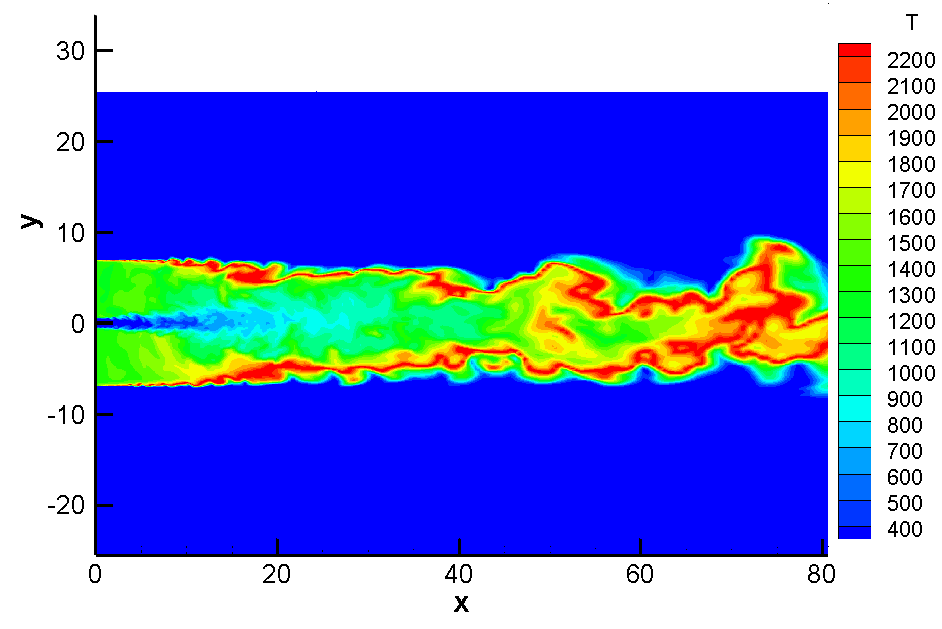
\includegraphics[width=\linewidth]{pic/flame.png}\\
				{\color{Green} Fig. 7 Jet flame}
			\end{center}
	\end{enumerate}

\vspace{-2cm}
\color{SaddleBrown} % SaddleBrown color for the conclusions to make them stand out
\section*{Conclusions}
	\color{DarkSlateGray}
	\begin{itemize}
	    \item
	    	Turbulent flamelet model shows better performance that traditional flame models.
	    \item
	    	$T_{max}$ curve solved in physical space has lower temperature, which is desired in practice.
	    \item 
	    	Finer vortex structures can be well resolved.
	    \vspace{10pt}
	\end{itemize}%

\nocite{*} % Print all references regardless of whether they were cited in the poster or not
\printbibliography

\section*{Acknowledgements}
	Special Thanks to Prof. Lipo Wang and Dr. Manuel Charlemagne. 

\end{multicols}
\end{document}


